%TODOS: macros for CUDA and SYCL to provide ™ throughout
%TODOS: check SYCL and CUDA terminology usage
%TODOS: clean up
%TODOS: check content


%%%%%%%%%%%%%%%%%%%%%%%
%
% The first command in your LaTeX source must be the \documentclass command.
\documentclass[sigconf]{acmart}

%
% defining the \BibTeX command - from Oren Patashnik's original BibTeX documentation.
\def\BibTeX{{\rm B\kern-.05em{\sc i\kern-.025em b}\kern-.08emT\kern-.1667em\lower.7ex\hbox{E}\kern-.125emX}}
    
% Rights management information. 
% This information is sent to you when you complete the rights form.
% These commands have SAMPLE values in them; it is your responsibility as an author to replace
% the commands and values with those provided to you when you complete the rights form.
%
% These commands are for a PROCEEDINGS abstract or paper.
\copyrightyear{2019}
\acmYear{2019}
\setcopyright{acmlicensed}
\acmConference[DHPCC++ '19]{Distributed \& Heterogeneous Programming for C/C++ (DHPCC++)}{May 13--15, 2019}{Boston, USA}
%\acmBooktitle{Woodstock '18: ACM Symposium on Neural Gaze Detection, June 03--05, 2018, Woodstock, NY}
%\acmPrice{15.00}
%\acmDOI{10.1145/1122445.1122456}
%\acmISBN{978-1-4503-9999-9/18/06}

%
% These commands are for a JOURNAL article.
%\setcopyright{acmcopyright}
%\acmJournal{TOG}
%\acmYear{2018}\acmVolume{37}\acmNumber{4}\acmArticle{111}\acmMonth{8}
%\acmDOI{10.1145/1122445.1122456}

%
% Submission ID. 
% Use this when submitting an article to a sponsored event. You'll receive a unique submission ID from the organizers
% of the event, and this ID should be used as the parameter to this command.
%\acmSubmissionID{123-A56-BU3}

%
% The majority of ACM publications use numbered citations and references. If you are preparing content for an event
% sponsored by ACM SIGGRAPH, you must use the "author year" style of citations and references. Uncommenting
% the next command will enable that style.
%\citestyle{acmauthoryear}

%
% end of the preamble, start of the body of the document source.
\usepackage{underscore}
\usepackage{listings}
\definecolor{keywordColor}{rgb}{0,0,0} %% black
\definecolor{stringColor}{rgb}{0.2, 0.2, 0.2}
\definecolor{commentColor}{rgb}{0.4,0.4,0.4} %% gray


\lstset{basicstyle=\normalsize\ttfamily, 
%framexleftmargin=2mm, framextopmargin=3mm, framexbottommargin=3mm, frame=shadowbox, 
%rulesepcolor=\color{gray}, aboveskip=0mm, belowskip=2mm, xleftmargin=2mm, 
keywordstyle=\color{keywordColor}\bfseries, stringstyle=\color{stringColor}, commentstyle=\color{commentColor}\slshape, showstringspaces=false, tabsize=2, escapechar={}, 
captionpos=b,caption=\lstname
,breaklines=true}

\lstdefinelanguage{C++11}{language=C++, morekeywords={alignas,alignof,char16_t,char32_t,constexpr, decltype, noexcept, nullptr, tatic_assert, thread_local, typeid}}
\lstdefinelanguage{Cuda}{language=C++11, morekeywords={__global__,__device__,__host__,__constant__,__shared__},
moredelim=[s][keywordstyle]{<<<}{>>>}}
\lstdefinestyle{C++11}{language=C++11,basicstyle=\normalsize\ttfamily}
\lstdefinestyle{Cuda}{language=Cuda,basicstyle=\normalsize\ttfamily}

\newcommand{\inputcode}[2]{\lstinputlisting[language=Cuda, label=#1, caption=#2]{#1}}
\newcommand{\inputsycl}[2]{\lstinputlisting[language=C++11, label=#1, caption=#2]{#1}}

\newcommand{\tcode}[1]{\texttt{#1}}
\newcommand{\intt}[1]{\texttt{#1}}
\newcommand{\nvidia}{NVIDIA\textsuperscript{\textregistered}}
\newcommand{\nsight}{Nsight\texttrademark{}}

\begin{document}

%
% The "title" command has an optional parameter, allowing the author to define a "short title" to be used in page headers.
\title{ReSYCLator: Transforming CUDA C++ source code into SYCL}

%
% The "author" command and its associated commands are used to define the authors and their affiliations.
% Of note is the shared affiliation of the first two authors, and the "authornote" and "authornotemark" commands
% used to denote shared contribution to the research.
\author{Tobias Stauber}
%\authornote{Both authors contributed equally to this research.}
\email{tobias.stauber@hsr.ch}
%\orcid{1234-5678-9012}
\author{Peter Sommerlad}
%\authornotemark[1]
\email{peter.sommerlad@hsr.ch}
\affiliation{%
  \institution{IFS Institute for Software at FHO-HSR Hochschule für Technik}
  \streetaddress{Oberseestrasse 10}
  \city{Rapperswil}
  \country{Switzerland}
  %\state{SG}
  \postcode{CH-8640}
}

%
% By default, the full list of authors will be used in the page headers. Often, this list is too long, and will overlap
% other information printed in the page headers. This command allows the author to define a more concise list
% of authors' names for this purpose.
%\renewcommand{\shortauthors}{Stauber , et al.}

%
% The abstract is a short summary of the work to be presented in the article.
\begin{abstract}
CUDA\texttrademark{} while very popular, is not as flexible with respect to target devices as OpenCL\texttrademark{}. 
While parallel algorithm research might address problems first with a CUDA C++ solution, those results are not easily portable to a target not directly supported by CUDA. 
In contrast, a SYCL\texttrademark{} C++ solution can operate on the larger variety of platforms supported by OpenCL.

ReSYCLator is a plug-in for Cevelop\cite{cevelop} an extension of Eclipse-CDT that bridges the gap between algorithm availability and portability, by providing automatic transformation of CUDA C++ code to SYCL C++. A first attempt basing the transformation on \nvidia's \nsight Eclipse CDT plug-in showed that \nsight's weak integration into CDT's static analysis and refactoring infrastructure is insufficient. Therefore, an own CUDA-C++ parser for Eclipse CDT was developed that is a sound platform for transformations from CUDA C++ programs to SYCL based on AST transformations.
\end{abstract}

%
% The code below is generated by the tool at http://dl.acm.org/ccs.cfm.
% Please copy and paste the code instead of the example below.
%
\begin{CCSXML}
<ccs2012>
<concept>
<concept_id>10011007.10011006.10011041.10011047</concept_id>
<concept_desc>Software and its engineering~Source code generation</concept_desc>
<concept_significance>500</concept_significance>
</concept>
<concept>
<concept_id>10011007.10011006.10011066.10011069</concept_id>
<concept_desc>Software and its engineering~Integrated and visual development environments</concept_desc>
<concept_significance>500</concept_significance>
</concept>
<concept>
<concept_id>10011007.10011006.10011073</concept_id>
<concept_desc>Software and its engineering~Software maintenance tools</concept_desc>
<concept_significance>300</concept_significance>
</concept>
</ccs2012>
\end{CCSXML}

\ccsdesc[500]{Software and its engineering~Integrated and visual development environments}
\ccsdesc[300]{Software and its engineering~Source code generation}
\ccsdesc[300]{Software and its engineering~Software maintenance tools}

%
% Keywords. The author(s) should pick words that accurately describe the work being
% presented. Separate the keywords with commas.
\keywords{CUDA C++, SYCL, C++, Eclipse CDT, integrated development environment}

%
% A "teaser" image appears between the author and affiliation information and the body 
% of the document, and typically spans the page. 
\begin{teaserfigure}
  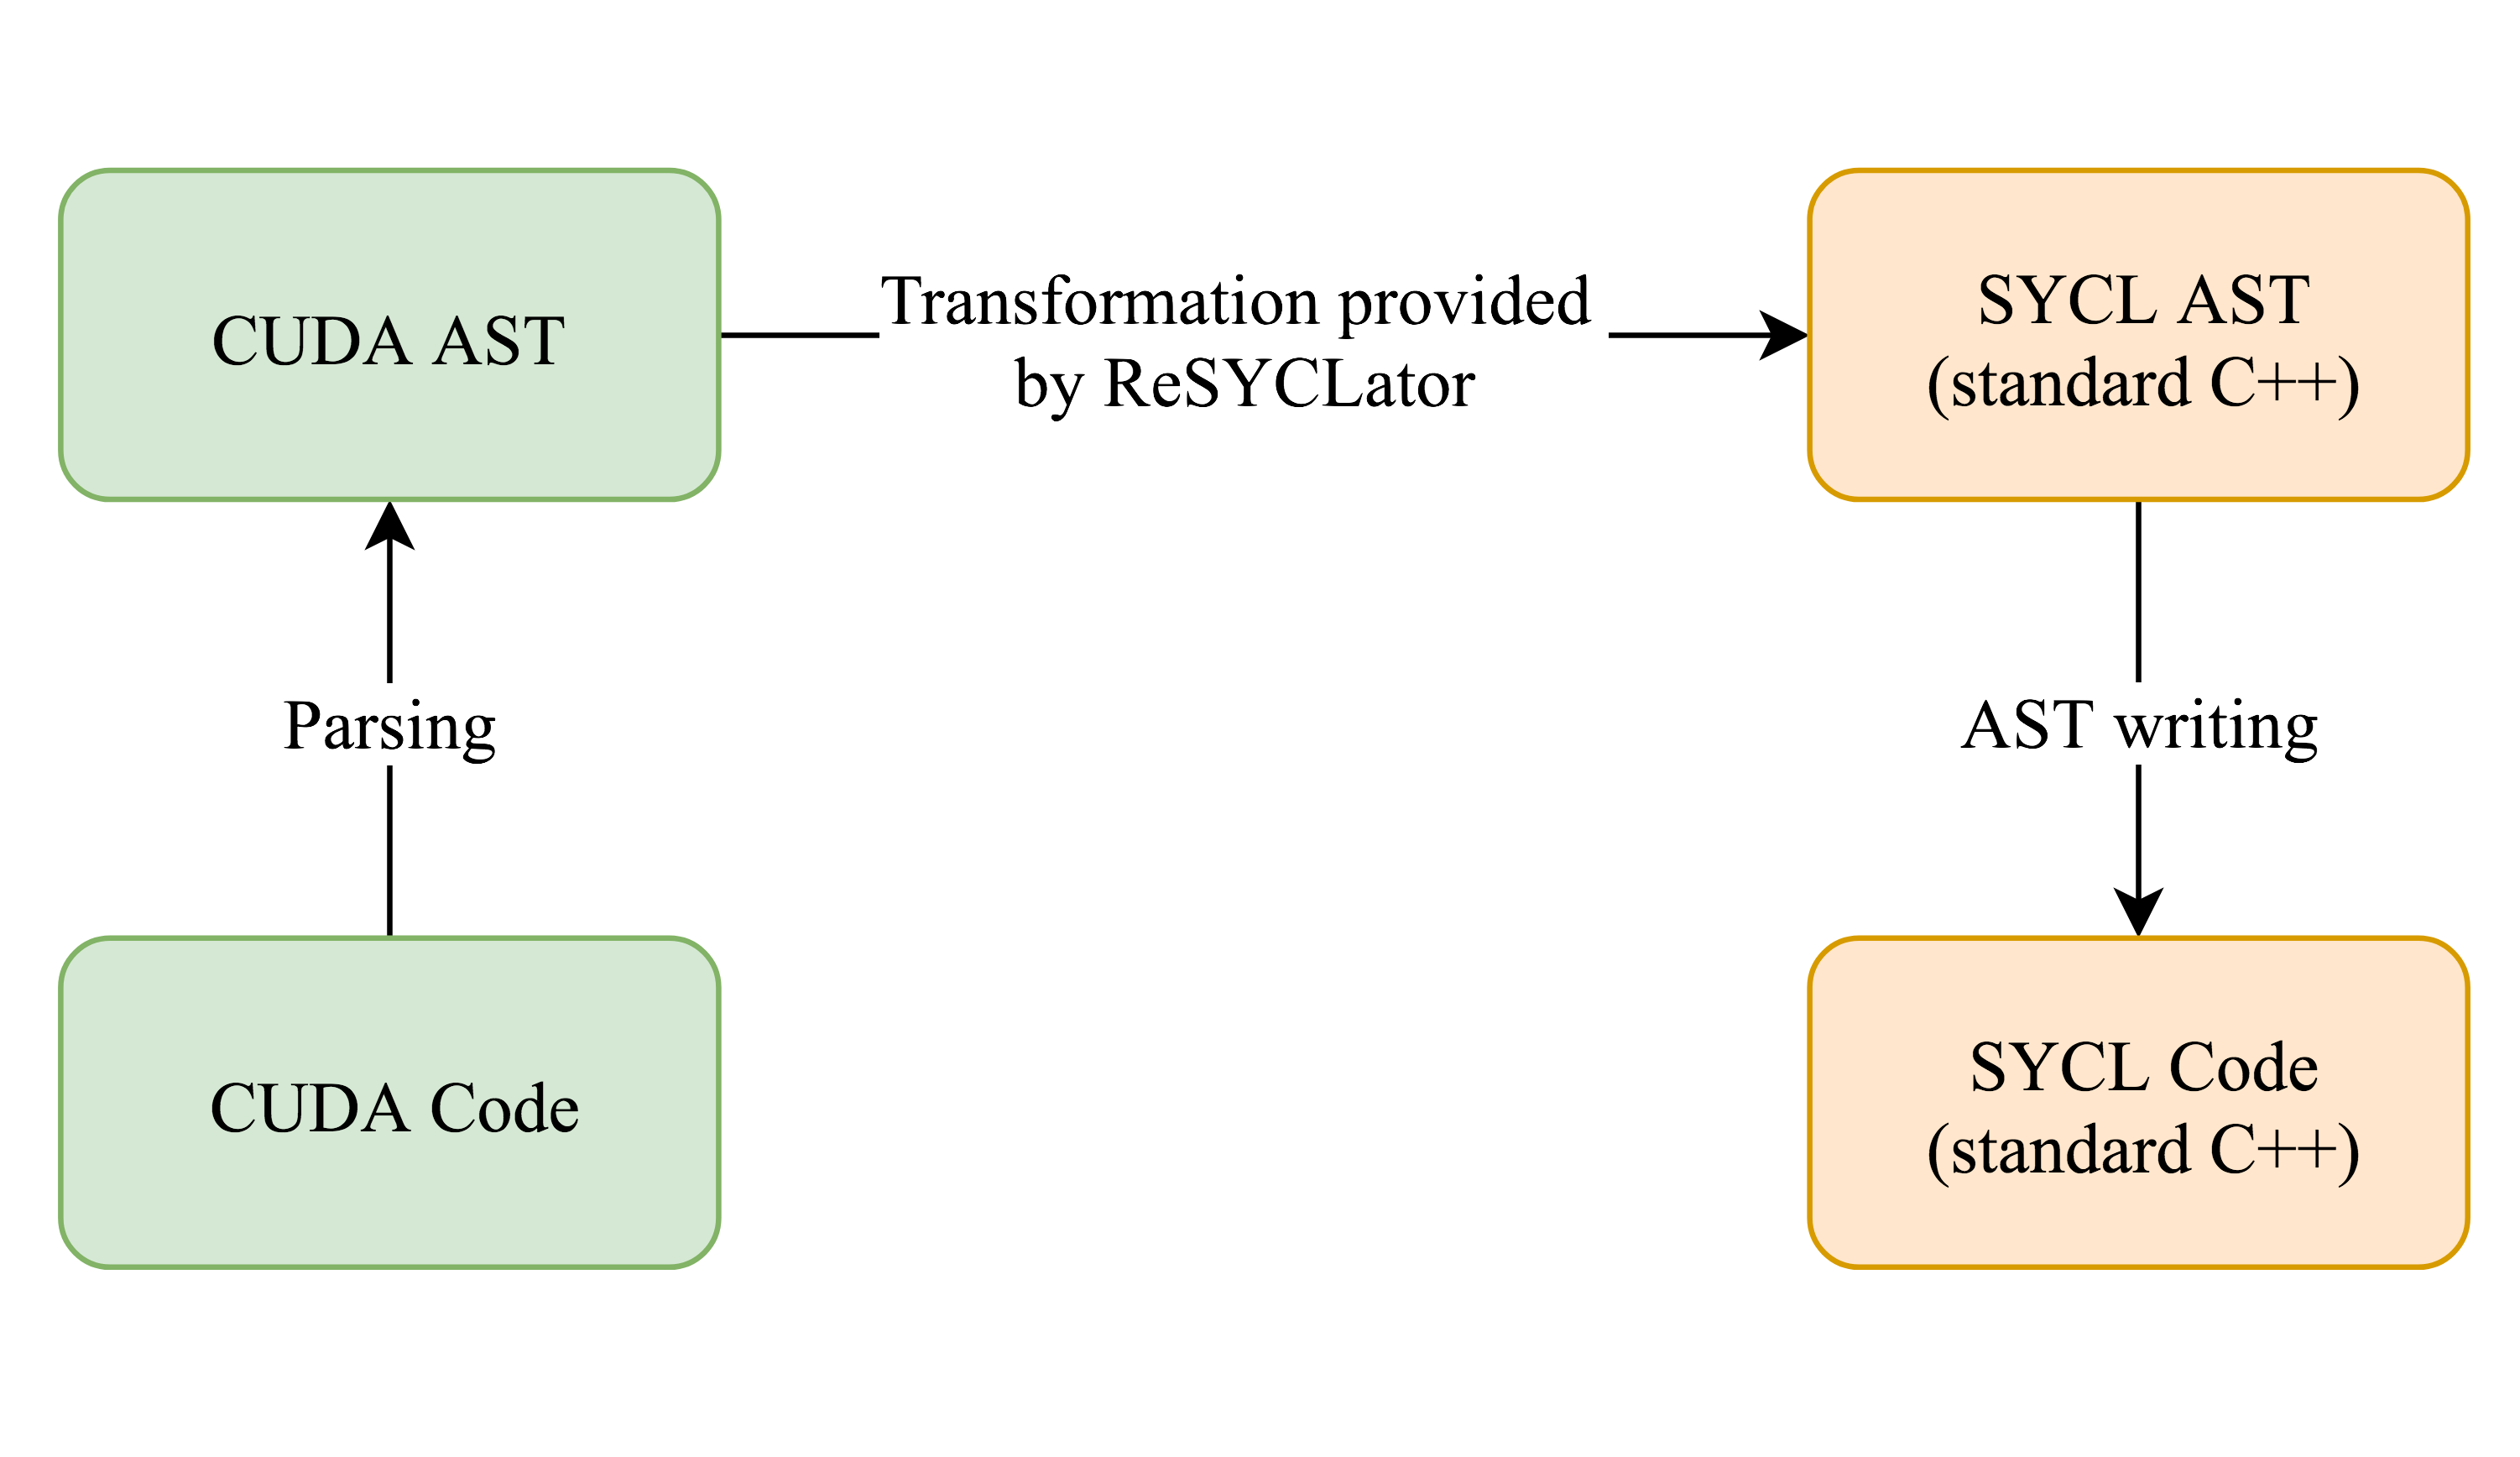
\includegraphics[width=\textwidth]{ReSYCLatorSchemaSimple}
  \caption{Transforming CUDA C++ code to SYCL using C++ AST Rewriting.}
  \Description{.}
  \label{fig:teaser}
\end{teaserfigure}

%
% This command processes the author and affiliation and title information and builds
% the first part of the formatted document.
\maketitle

\section{Introduction}

\nvidia's CUDA language is very popular but in addition to being bound to devices from a single vendor also introduces special syntax to C respectvely C++ for kernel function calls. This limits CUDA support in integrated development environments (IDEs) to what is provided by \nvidia, such as the \nsight plug-in for Eclipse CDT. However, working with a single source language and its relatively long availability makes it still attractive for developers, such as in parallel algorithm research.

The vendor lock-in is a reason why some industries would like to to switch to more open solutions that allow more heterogeneous target hardware. OpenCL itself also has a long history, but its classic separate compilation model of kernels, e.g., as strings in the host language passed to the run-time compiler, is a limiting factor in IDE support. The quite recently developed SYCL circumvents the limitations of CUDA and OpenCL by integrating heterogeneous parallel computation in standard C++ syntax.

With the plethora of existing CUDA parallel algorithm implementations it would be great to ease their porting to SYCL to mitigate the vendor lock-in and to allow additional heterogeneous platforms, such as FPGAs to run them.

\subsection{Institute for Software's history in Refactoring}
Our institute has a long history in implementing refactoring tools for Eclipse-based IDEs. We started out more than a decade ago to implement refactoring support for Eclipse CDT, such as AST-rewriting \cite{Graf2007}, heuristics for keeping the transformed code as close to its original representation, such as keeping comments around\cite{Sommerlad2008}, and also worked on source-to-source transformation of sequential C++ to parallel C++ including generating C++ source code targeting FPGAs in the EU-FP7 REPARA project
\cite{repara2016} \cite{repara2016a}. The result of our work on better supporting C++ modernization is currently made available through the free-to-use IDE Cevelop\cite{cevelop}

\section{CUDA syntax to be transformed}
The underlying concepts of CUDA as well as OpenCL/SYCL are not inherently different. That makes transformation feasible. However, manual transformation can be very tedious.
Here we give a brief overview of key elements of CUDA syntax that will be transformed. Unfortunately, at the time of this writing, no formal specification of CUDA syntax is available in contrast to standard C++\cite{isocpp}, so what is described here is derived from  the CUDA programming guide\cite{CUDACProgGuide} that presents the NVCC CUDA dialect.

\subsection{Marking CUDA Kernels}
Kernel functions in CUDA are marked with the following specifiers:
\begin{description}
\item[\tcode{__host__}] function is executable on the host CPU (redundant, unless combined with \tcode{__device__})
\item[\tcode{__global__}] kernel function that is executable on the GPU device and can be called with the special call syntax
\item[\tcode{__device__}] function executable and callable only on the device, unless combined with \tcode{__host__}
\end{description}
These identifiers are implemented as macros, which makes detecting them in the parsed AST already a challenge. Similar specifiers are used for memory space designation (\tcode{__device__}, \\\tcode{__constant__}, \tcode{__shared__}). 


\subsection{Invoking Kernels}
    For calling a kernel, there is a special syntax. This syntax consists of \intt{<{}<{}<} to start the launch-parameter list, and \intt{>{}>{}>} to close it (Listing~\ref{invoke-example.cpp}).
    
    \inputcode{invoke-example.cpp}{Special CUDA kernel invocation syntax}
    
    The first mandatory argument, \intt{grid_dimensions}, is of type \intt{int}, \intt{uint3}, or \intt{dim3}, and defines how many blocks are contained in the grid in each dimension (x, y, z). %(\fanref{see}{cuda:details:fig:cudagrid}).
    
    The second argument, \intt{block_dimensions}, is also mandatory, and of type \intt{int}, \intt{uint3}, or \intt{dim3}. It is used to define how many threads are there per dimension in a block. %(\fanref{see}{cuda:details:fig:cudablock}).
    
    The number of bytes of shared memory allocated for each block in the grid are passed as an optional argument \intt{size_t} (\intt{bytes_of_shared_mem}). 
    
    The optional argument \intt{stream} tells the CUDA on which stream this kernel should be run. This value must be of type \intt{cudaStream_t} and defaults to the default-stream if omitted.

    The concept of CUDA streams is not handled yet, but it can be transformed to SYCL queues.


\subsection{Special Indicdes}
In a CUDA kernel, each running thread has a set of built-in variables allowing to calculate the current block's position in the grid (\tcode{blockIdx}) and a thread's position in the block (\tcode{threadIdx}). Both dimensions are given by the special CUDA arguments of a kernel call. The member selectors \tcode{.x}, \tcode{.y}, \tcode{.z} allow indexing relative to each thread running a kernel.

\section{Transforming CUDA kernels to SYCL kernels}
The information on CUDA kernel functions, memory management operations (omitted above), and kernel implementations needs to be detected in CUDA source code and transformed to corresponding SYCL mechanisms in C++. Most of the remaining plain C++ code can be taken literally.
 
\subsection{Adjusting kernel function signatures}
A first step in the transformation is to find CUDA kernel function definitions and declarations, i.e., by looking for those that have the attribute global attached, because the \tcode{__global__} macro is expanded to (\tcode{__attribute__((global))}) in the case of the GCC compiler as in Listing~\ref{cudadecl.cpp}. Using the Microsoft Visual Studio Compiler toolchain the macro would be expanded to \tcode{__declspec(__global__)}.
\inputcode{cudadecl.cpp}{Declaring a CUDA kernel}

In the C++ AST of Eclipse CDT macros are expanded, while also the original source code with the unexpanded macro is referred by it. 
Macros are one of the aspects that makes AST-based code transformations tricky in C++. 
However, the AST nodes representing the CUDA kernel specifier get removed. 
Then the CUDA parameter declarations need to be extended to include the SYCL-specific \tcode{nd_item} dimension parameter as their first parameter. The dimension template argument of \tcode{nd_item} is introduced by transforming the function declaration into a template function with an integer template parameter. 
As a remaining step the pointer parameters of a typical CUDA kernel, need to be mapped to SYCL accessors (Listing~\ref{sycldecl2.cpp}) or SYCL global pointers(Listing~\ref{sycldecl1.cpp}). 
The latter is used in the transformation, because it allows a more direct mapping of the kernel function body. 
However, in the future a SYCL-specific refactoring from global pointer parameters to accessors could be provided using Cevelop's refactoring infrastructure. Such a refactoring could be beneficial also for existing or manually transformed SYCL code.
\inputsycl{sycldecl1.cpp}{SYCL declaration with global pointers}
\inputsycl{sycldecl2.cpp}{SYCL declaration with accessors}

\subsection{Transforming kernel function bodies}
After the kernel signature has been adjusted to SYCL, the actual kernel code needs to be transformed. One major substitution to take place, is to translate the CUDA-specific index variables (\tcode{threadIdx}, \tcode{blockIdx}) and dimension variables (\tcode{blockDim}, \tcode{gridDim}) to corresponding accesses via the SYCL \tcode{nd_item} parameter. Each CUDA index and dimension variable provides three member accessors (x, y, z) that map to SYCL dimension indices 0, 1, 2 respectively. For the rest of the mapping see Table~\ref{tab:mapping} where DIM denotes member and its corresponding index respectively.
\begin{table}[htp]
\begin{center}\begin{tabular}{|l|l|}
\hline
 CUDA variable & SYCL \tcode{nd_item} call \\\hline
  \tcode{threadIdx.DIM} & \tcode{item.get_local_id(DIM)} \\\hline
   \tcode{blockIdx.DIM} & \tcode{item.get_group(DIM)} \\\hline
    \tcode{blockDim.DIM} & \tcode{item.get_local_range(DIM)} \\\hline
     \tcode{gridDim.DIM} & \tcode{item.get_local_id(DIM)} \\\hline
      \end{tabular} 
      \caption{Mapping CUDA variables to SYCL nd_item member functions}
\end{center}
\label{tab:mapping}
\end{table}
      
Taking the original CUDA implementation from Listing~\ref{cudamult.cpp} will result in the following transformed SYCL kernel function in Listing~\ref{syclmult.cpp}. Note that, due to a SYCL compiler warning, array index operator uses on pointers was translated to explicit pointer arithmetic. In the future this cludge might no longer be required to produce valid code.
\inputcode{cudamult.cpp}{CUDA matrix multiplication kernel}
\inputsycl{syclmult.cpp}{Transformed SYCL kernel function}

\section{Transforming CUDA kernel call site}
A typical call site of a CUDA kernel consists of the following parts:
\begin{itemize}
\item pointer definitions for memory blocks to be allocated
\item preparation of memory through cudaMalloc calls
\item initializing kernel input data
\item preparing kerne grid dimensions depending on data size and layout, if not fixed
\item the CUDA kernel call (see Listing~\ref{invoke-example.cpp})
\item synchronizing with the device
\item obtaining the results
\item freeing the memory
\end{itemize}
The example program in Listing~\ref{cuda-main.cpp} shows this and compares a CPU matrix multiplication result with the GPU results.

All these parts have to be adapted to the concepts and syntax of SYCL. Fortunately, some of the parts can be eliminated in total, such as the explicit freeing of memory, because SYCL employs the C++ scope-based resource management idiom with automatic clean-up when leaving a scope.

\subsection{SYCL memory buffer set up}
As one can see in Listing~\ref{cuda-main.cpp} a typical CUDA program needs to call allocation and deallocation functions symmetrically to provide memory for device use. This is not considered a relevant style in C++, where the RAII pattern(resource-acquisition is initialization)--also called scope-bound resource management (SBRM) provides a cleaner and less error-prone mechanism. So the definition of pointers and \tcode{cudaMalloc} and \tcode{cudaFree} calls are replaced by SYCL buffers, that automatically manage memory allocation, transfer to and from, and synchronization with the computing device.

As an example, for the usage of one of the input matrices (A) the lines declaring the pointer, allocating device memory, synchronizing results as well as freeing the memory again as the excerpt from Listing~\ref{cuda-main.cpp} in Listing~\ref{cuda-main-a.cpp}, get replaced by the corresponding code that is synthesized from the CUDA code in Listing~\ref{sycl-main-a.cpp}. Note, that in contrast to cudaMalloc call that allocates bytes, the SYCL buffer variable definition automatically takes the size of the element type into account. The refactoring detects if the expression can just drop the \tcode{sizeof} expression from a multiplication. In case of a more complex, or simpler size computation the division by \tcode{sizeof(elementtype)} is explicitly introduced.

\inputcode{cuda-main-a.cpp}{Setting up and cleaning up CUDA input data.}
\inputsycl{sycl-main-a.cpp}{SYCL buffer declaration replaces all lines in Listing~\ref{cuda-main-a.cpp}}

\subsection{SYCL memory accessors from CUDA pointer accesses}
\label{SYCL:accessors}
The example code in Listing~\ref{cuda-main.cpp} contains nested loops initializing the input matrices. For simplicity, this loop does two dimensional index transformation manually in the allocated area using the pointers. 
Since SYCL accesses all buffer memory through SYCL accessors for such an access corresponding accessor objects have to be created. 
It is important that these accessor objects are defined in a as local as possible scope, because their lifetime is used to synchronize between host and kernel access to the underlying buffer. 
Because the latter is quite expensive, it is also important that the accessors to a SYCL buffer are not defined within close loops. 
Therefore, the transformation will introduce a scope surrounding the initialization loops and defines two accessor variables in that newly introduced scope. The accessor variables' names are taken from the buffer name and prefixed with "\tcode{acc_}". 
This is a situation where AST-based transformations shine, because the AST subtree consisting of the usages is put into the newly introduced compound statement. 
You can also see the comment-retainment heuristic in action from \cite{Sommerlad2008}, because the comment associated with the outer for loop is also attached in front of the new compound statement.

Furthermore, the index accesses through the original pointer variables, e.g., \tcode{d_A}, need to be adjusted to use the newly introduced accessor variable \tcode{acc_d_A}. The transformed code for the loops filling matrices A and B from Listing~\ref{cuda-main.cpp} is shown in Listing~\ref{sycl-main-init.cpp}.
\inputsycl{sycl-main-init.cpp}{Introducing scope for SYCL accessors}


The underlying scope-introduction algorithm employs slicing and scope matching to find or introduce a minimal scope for all CUDA-pointer based accesses. This avoids blocking SYCL buffer access from the kernel, because an accessor is still alive. At the end of its lifetime towards the end of the scope, a SYCL accessor releases its lock on the memory region managed by its associated SYCL buffer. From the example in Listing~\ref{cuda-main.cpp} a similar transformation would happen for the section commented with "Compare the results".

\subsection{Transforming a CUDA kernel call to a SYCL compute-queue submission} 

In contrast to the relatively simple CUDA kernel call syntax, activating a kernel in SYCL is a bit more elaborated, because it requires introducing a compute queue the kernel is submitted with. The special arguments to a CUDA kernel call specifying the underlying grid and block dimensions that are computed need to be mapped to SYCL's \tcode{nd_range} values. The CUDA types for dimensions allows a bit more flexibility, such as changing the values after initialization that complicates the mapping. This results in a slightly complicated determination of the SYCL range value, that needs to slice the code backwards from the CUDA kernel call to see the computed \tcode{dim3} dimensions, if not given as literals. The details of this algorithm are omitted for brevity here (\cite{stauberCUDASYCL2018}).

Each CUDA kernel call, such as the one in Listing~\ref{cuda-call.cpp} is replaced by a newly introduced compound statement that provides a local scope for the required SYCL objects creating a compute queue and submitting the kernel to it. 
The \tcode{submit()} call takes a lambda expression that consists of creating the necessary accessor objects, like shown in section~\ref{SYCL:accessors}. Next the lambda calls parallel_for on the handler objects passing the dimensions and accessors to the actual kernel, which is again wrapped in a lambda resulting in the code given in Listing~\ref{sycl-submit.cpp}. The forward-declared class type used as a template argument to parallel_for is used by SYCL as a unique identifier. So this name (abbreviated here as \tcode{class matrixMul_f0}) must be synthesized in a way that guarantees uniqueness. 
\inputcode{cuda-matrix-call.cpp}{Kernel call to be transformed}
\inputsycl{sycl-submit.cpp}{Submitting transformed kernel}

This concludes up the transformations required to map CUDA C++ code to SYCL: transforming kernels, mapping memory management and access, calling kernels. In some areas the resulting code gets simpler, especially with respect to resource management. In some others, such as calling the kernel, the CUDA "magic" is replaced by the more transparent but elaborated SYCL compute queue submission. The complete converted program can be seen in Listing~\ref{sycl-matrix-main.cpp} in the Appendix. The required SYCL header include directives are also inserted automatically.

\section{Tooling architecture}
To complete the paper, a brief overview of the underlying tooling architecture is given. The initial prototype attempted to use the \nsight{} Eclipse CDT plug-in and attempted to build the transformation on top of it as given in Figure~\ref{fig:protoarch}. While a working example transformation could be created, that "solution" showed that the internal parsing infrastructure and its relatively inaccessibility were not up to what is needed for sound code analysis and transformation. 
\begin{figure}[h]
  \centering
  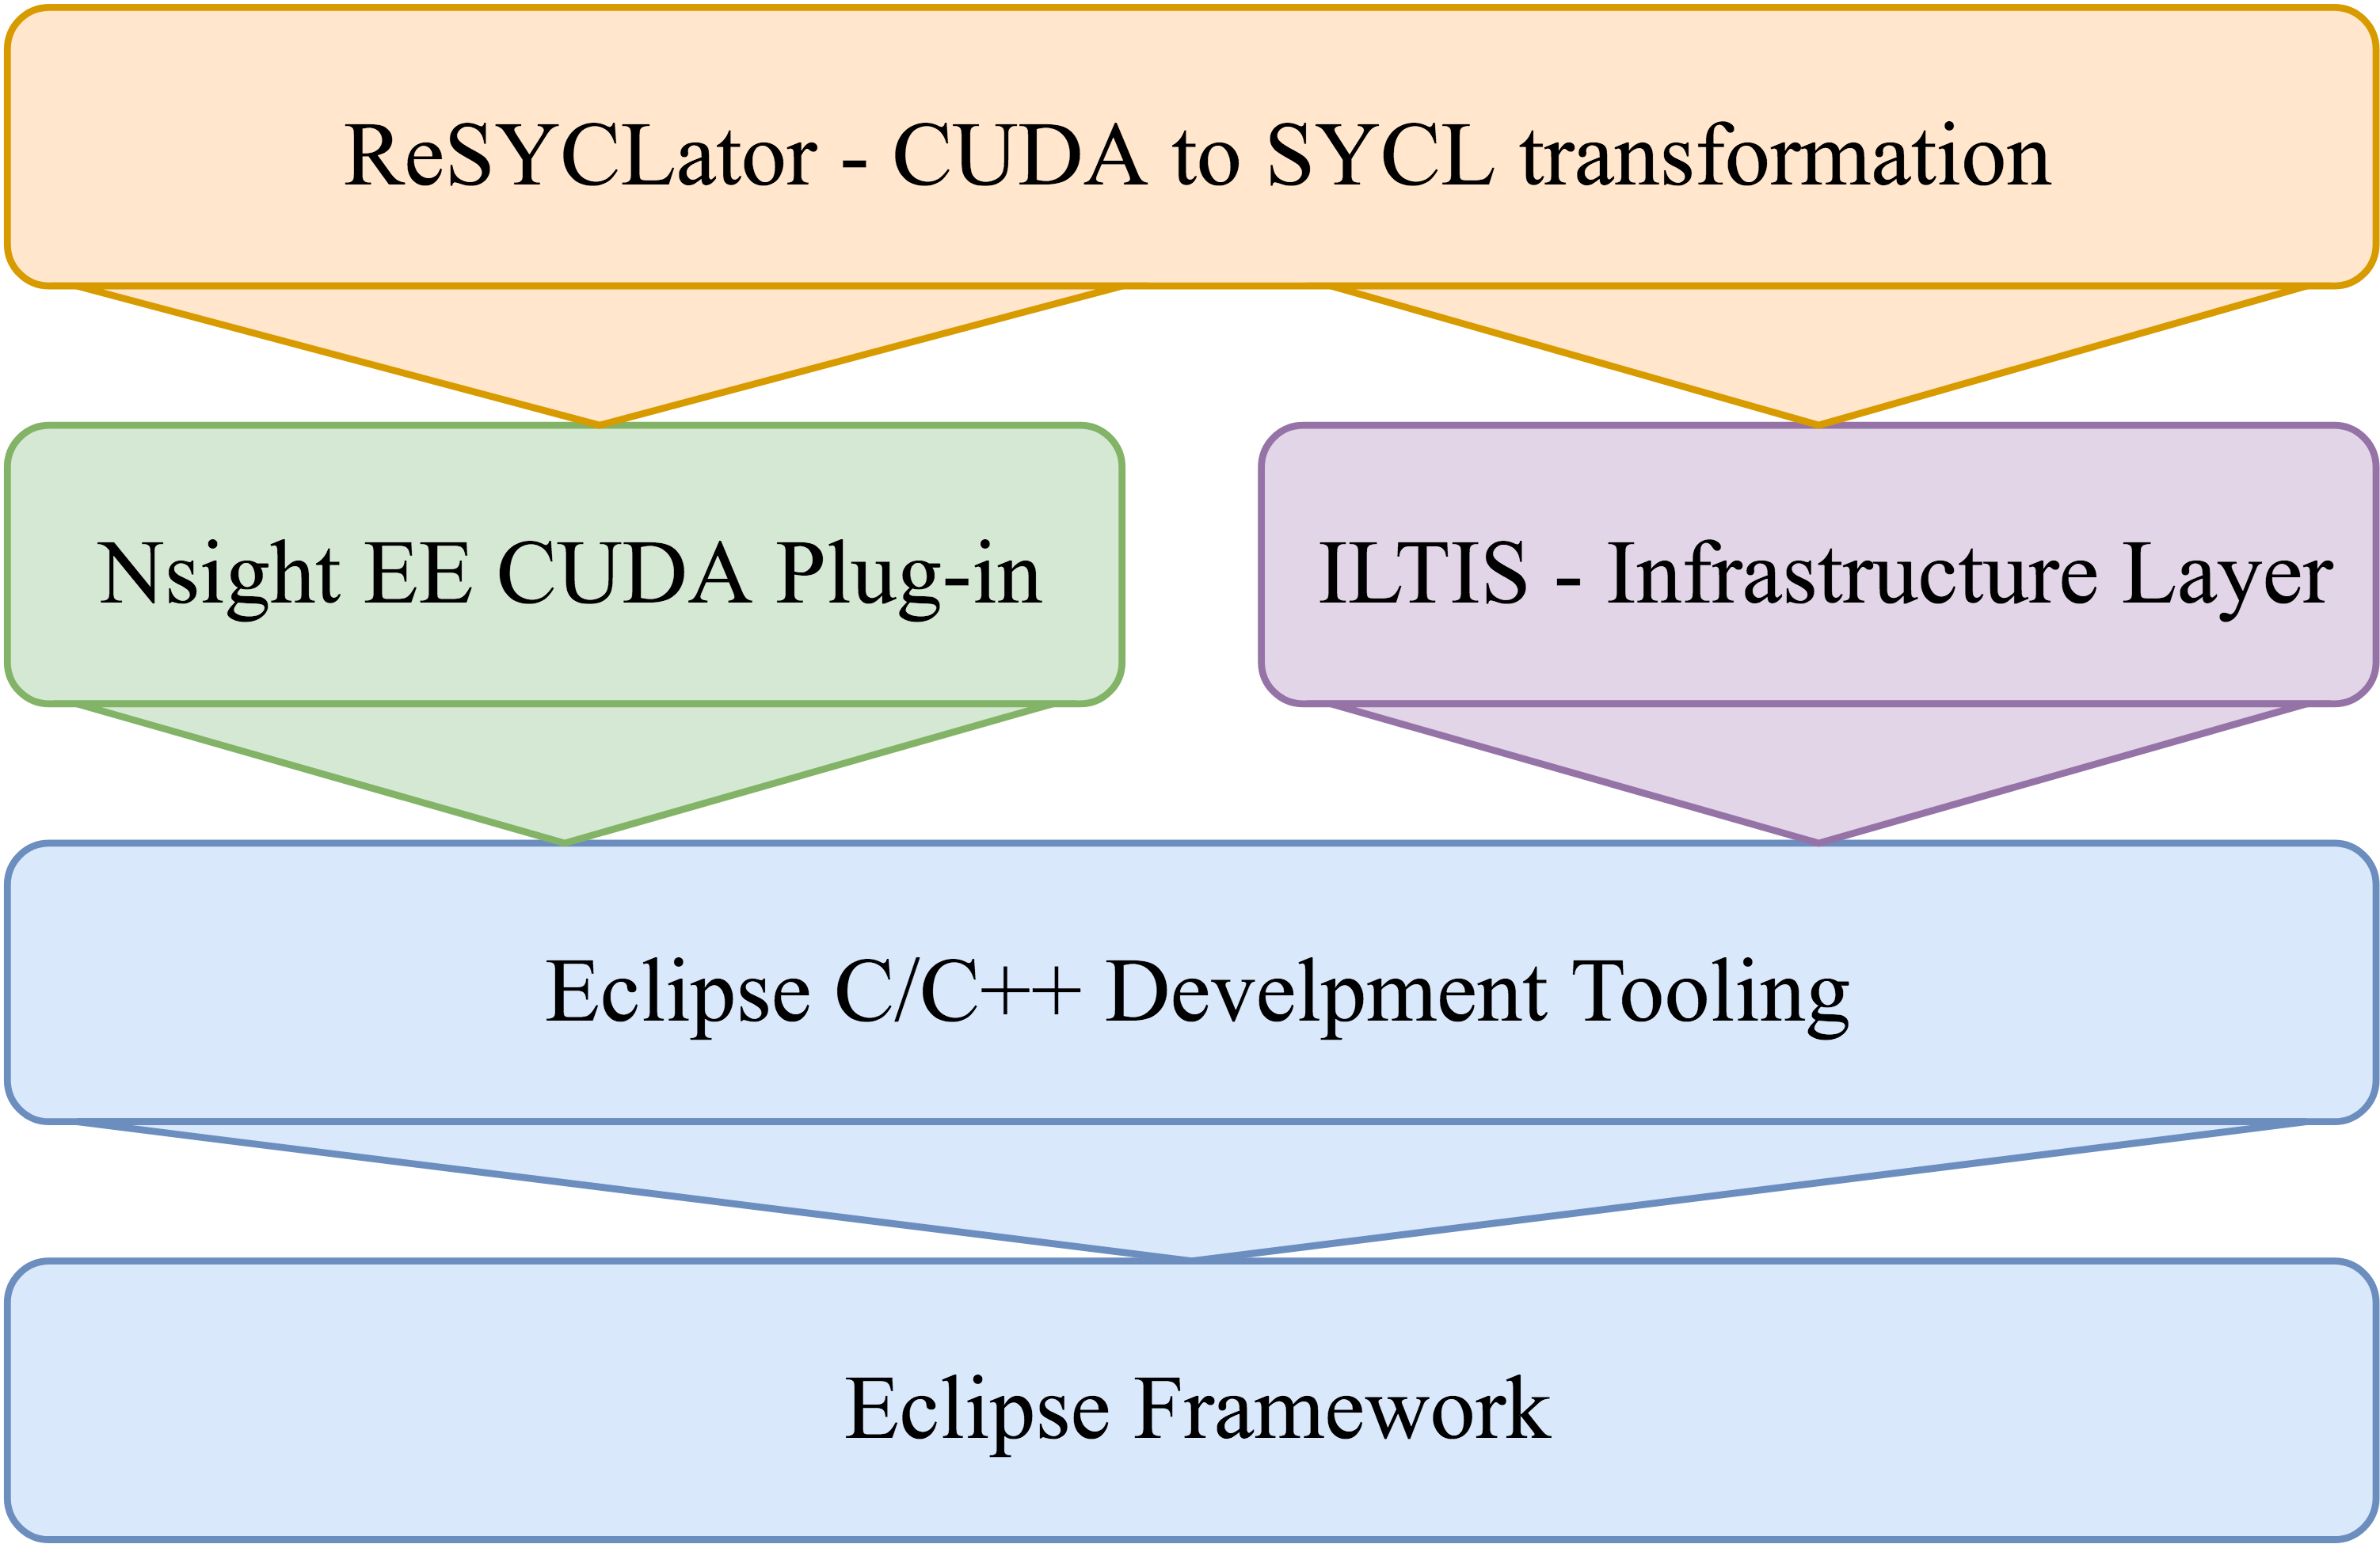
\includegraphics[width=\linewidth]{SimpleArchitectureNsight}
  \caption{Architectural overview initial prototype.}
  %\Description{.}
  \label{fig:protoarch}
\end{figure}

The second attempt created a CUDA parsing infrastructure (CRITTER) and embedded this into the existing Eclipse CDT C++ AST and transformation infrastructure\cite{stauberCRITTER2019}. The ILTIS layer \cite{stauberIltis2018} abstracts many CDT internals required to ease porting AST transformation plug-ins to newer CDT releases. With that basis the ReSYCLator CUDA to SYCL transformation is on a much sounder platform for future extensions as shown in Figure~\ref{fig:resultarch}.

\begin{figure}[h]
  \centering
  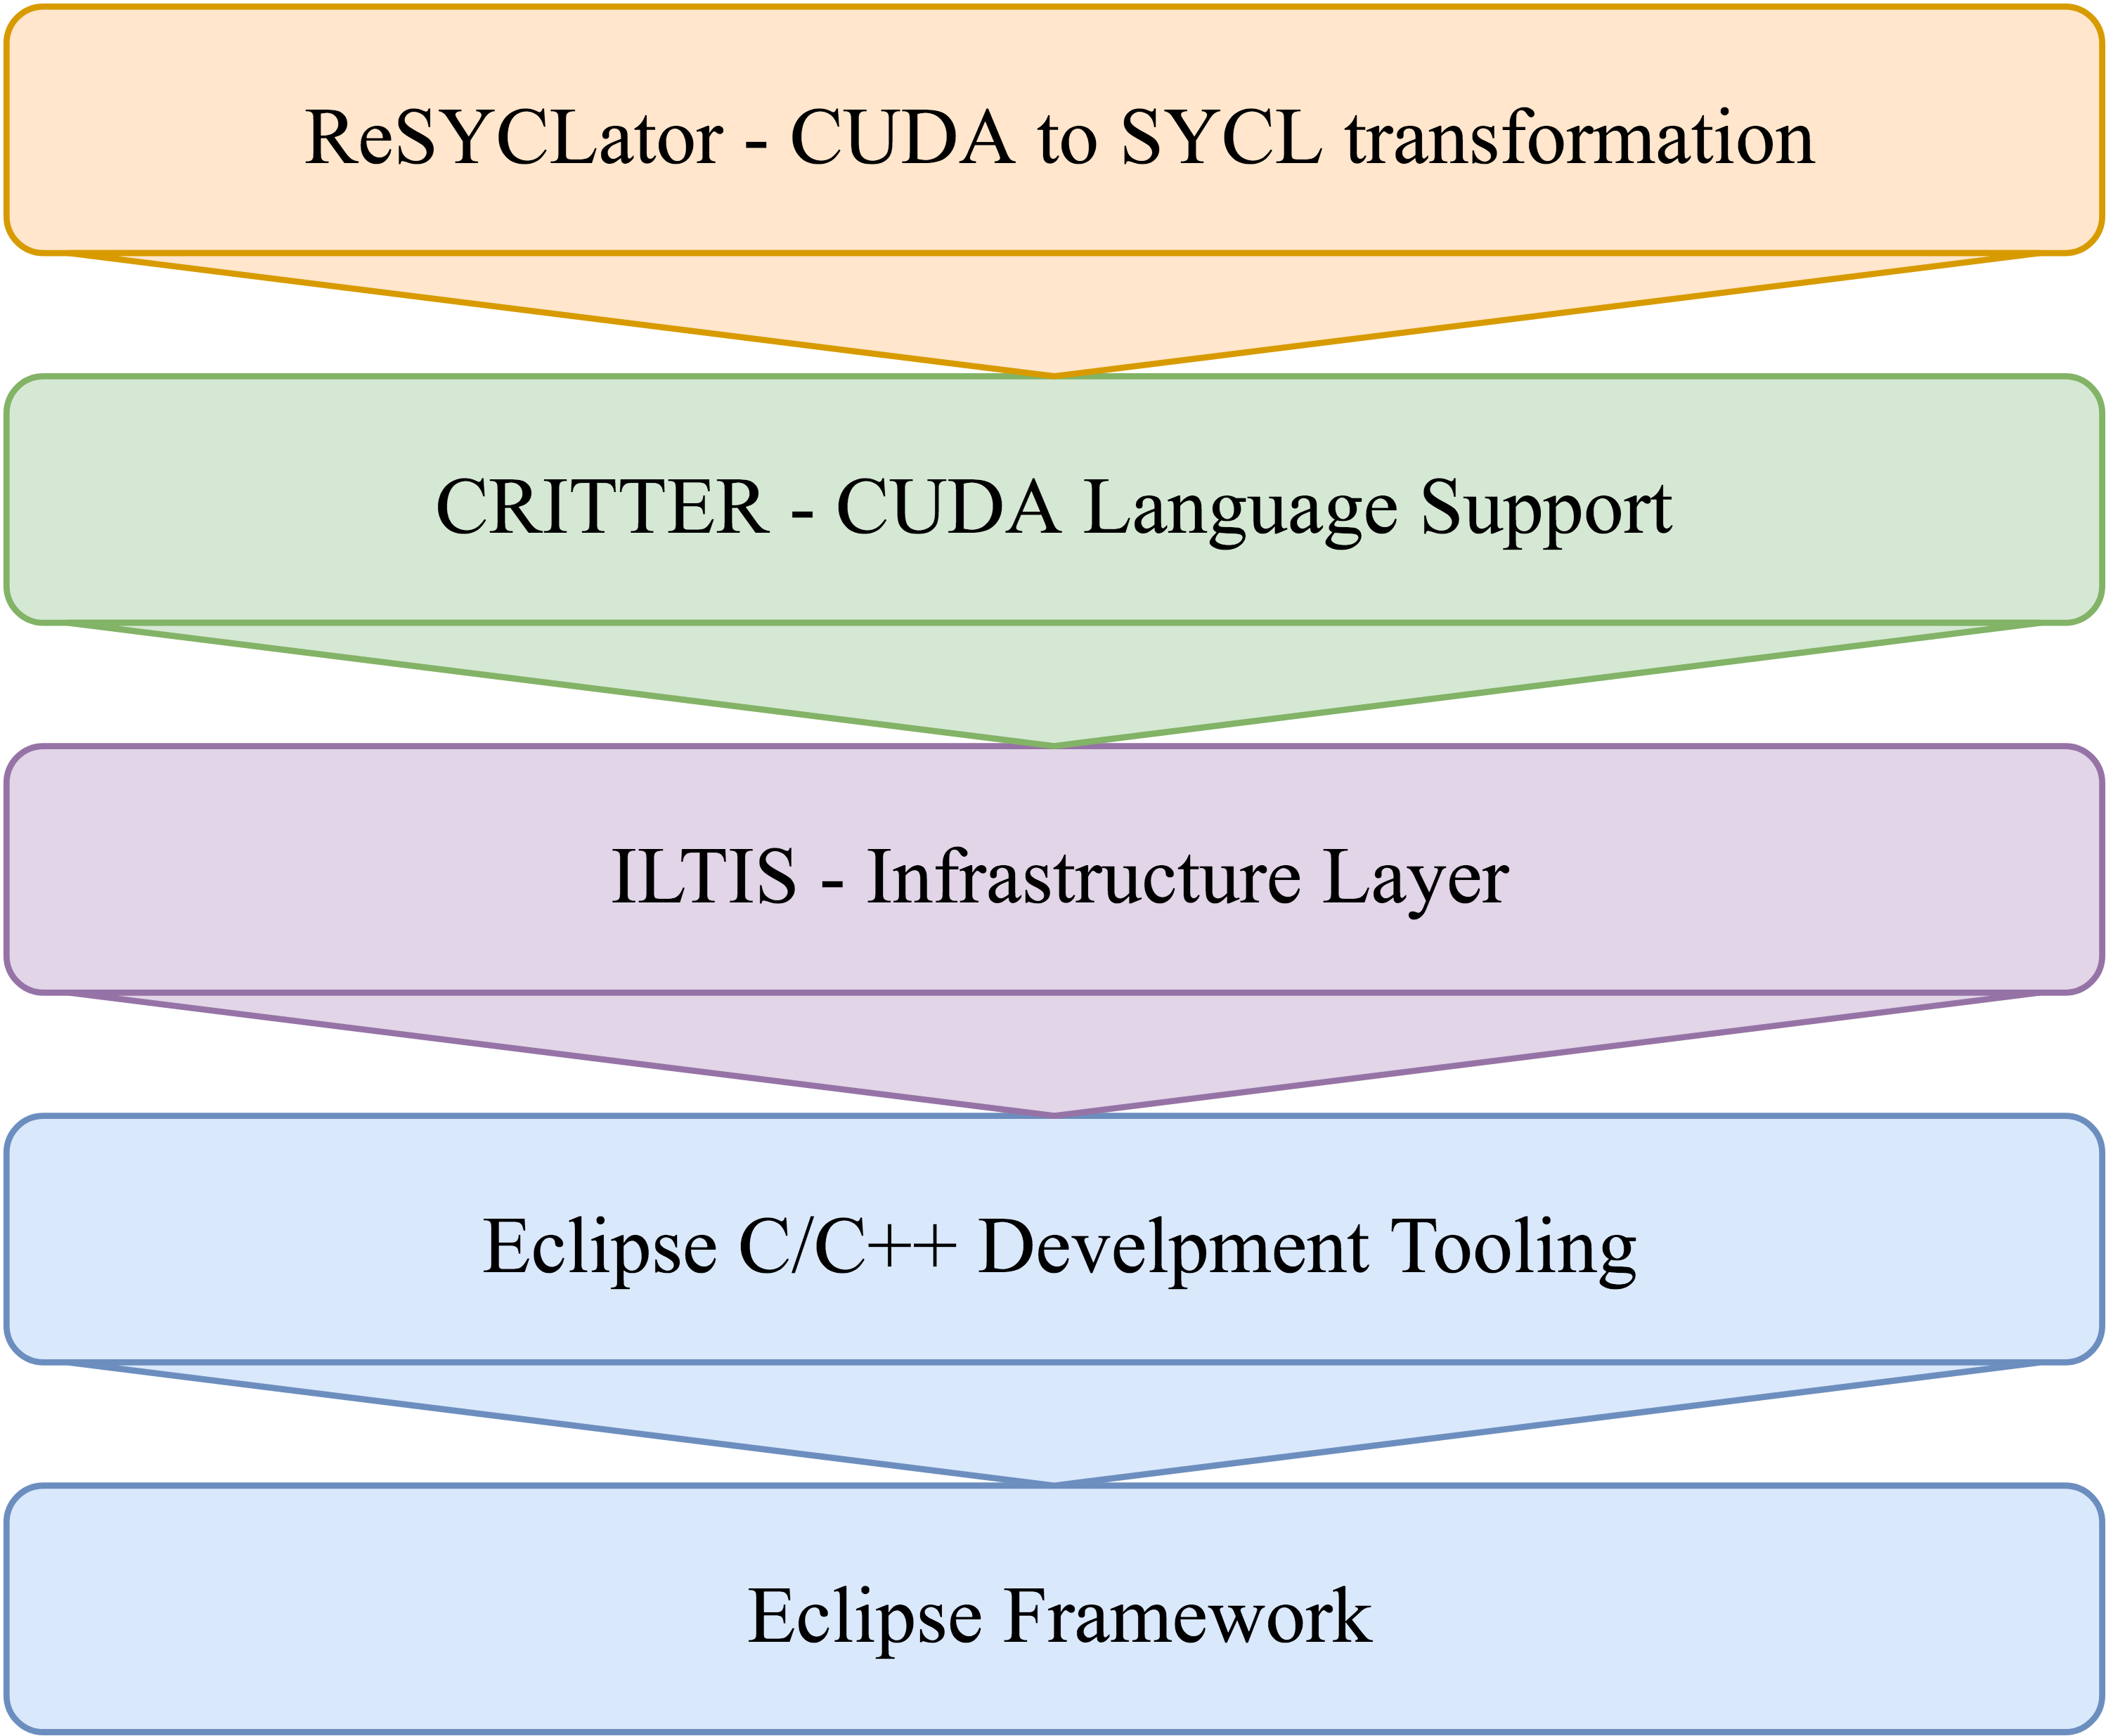
\includegraphics[width=\linewidth]{SimpleArchitectureCRITTER}
  \caption{Architectural overview relying on own CUDA parser.}
  %\Description{.}
  \label{fig:resultarch}
\end{figure}

The following Figure~\ref{fig:toolarch} shows the internal dependencies/extension point implementations of the individual Eclipse components created during this project. Note the output specified as "SYCL AST" is not actually a component. The Eclipse framework and Eclipse CDT provide the right hand facilities. The CUDA C++ parser is build by extending Eclipse CDT's C++ parser and AST with additional syntax. To fit everything in the workspace environment of Eclipse CDT, CUDA language support infrastructure needed to be created in addition to the CUDA C++ parser. This allows to seamlessly work with CUDA sources as well as with SYCL C++ sources within the same Eclipse workspace seamlessly.


\begin{figure}[h]
  \centering
  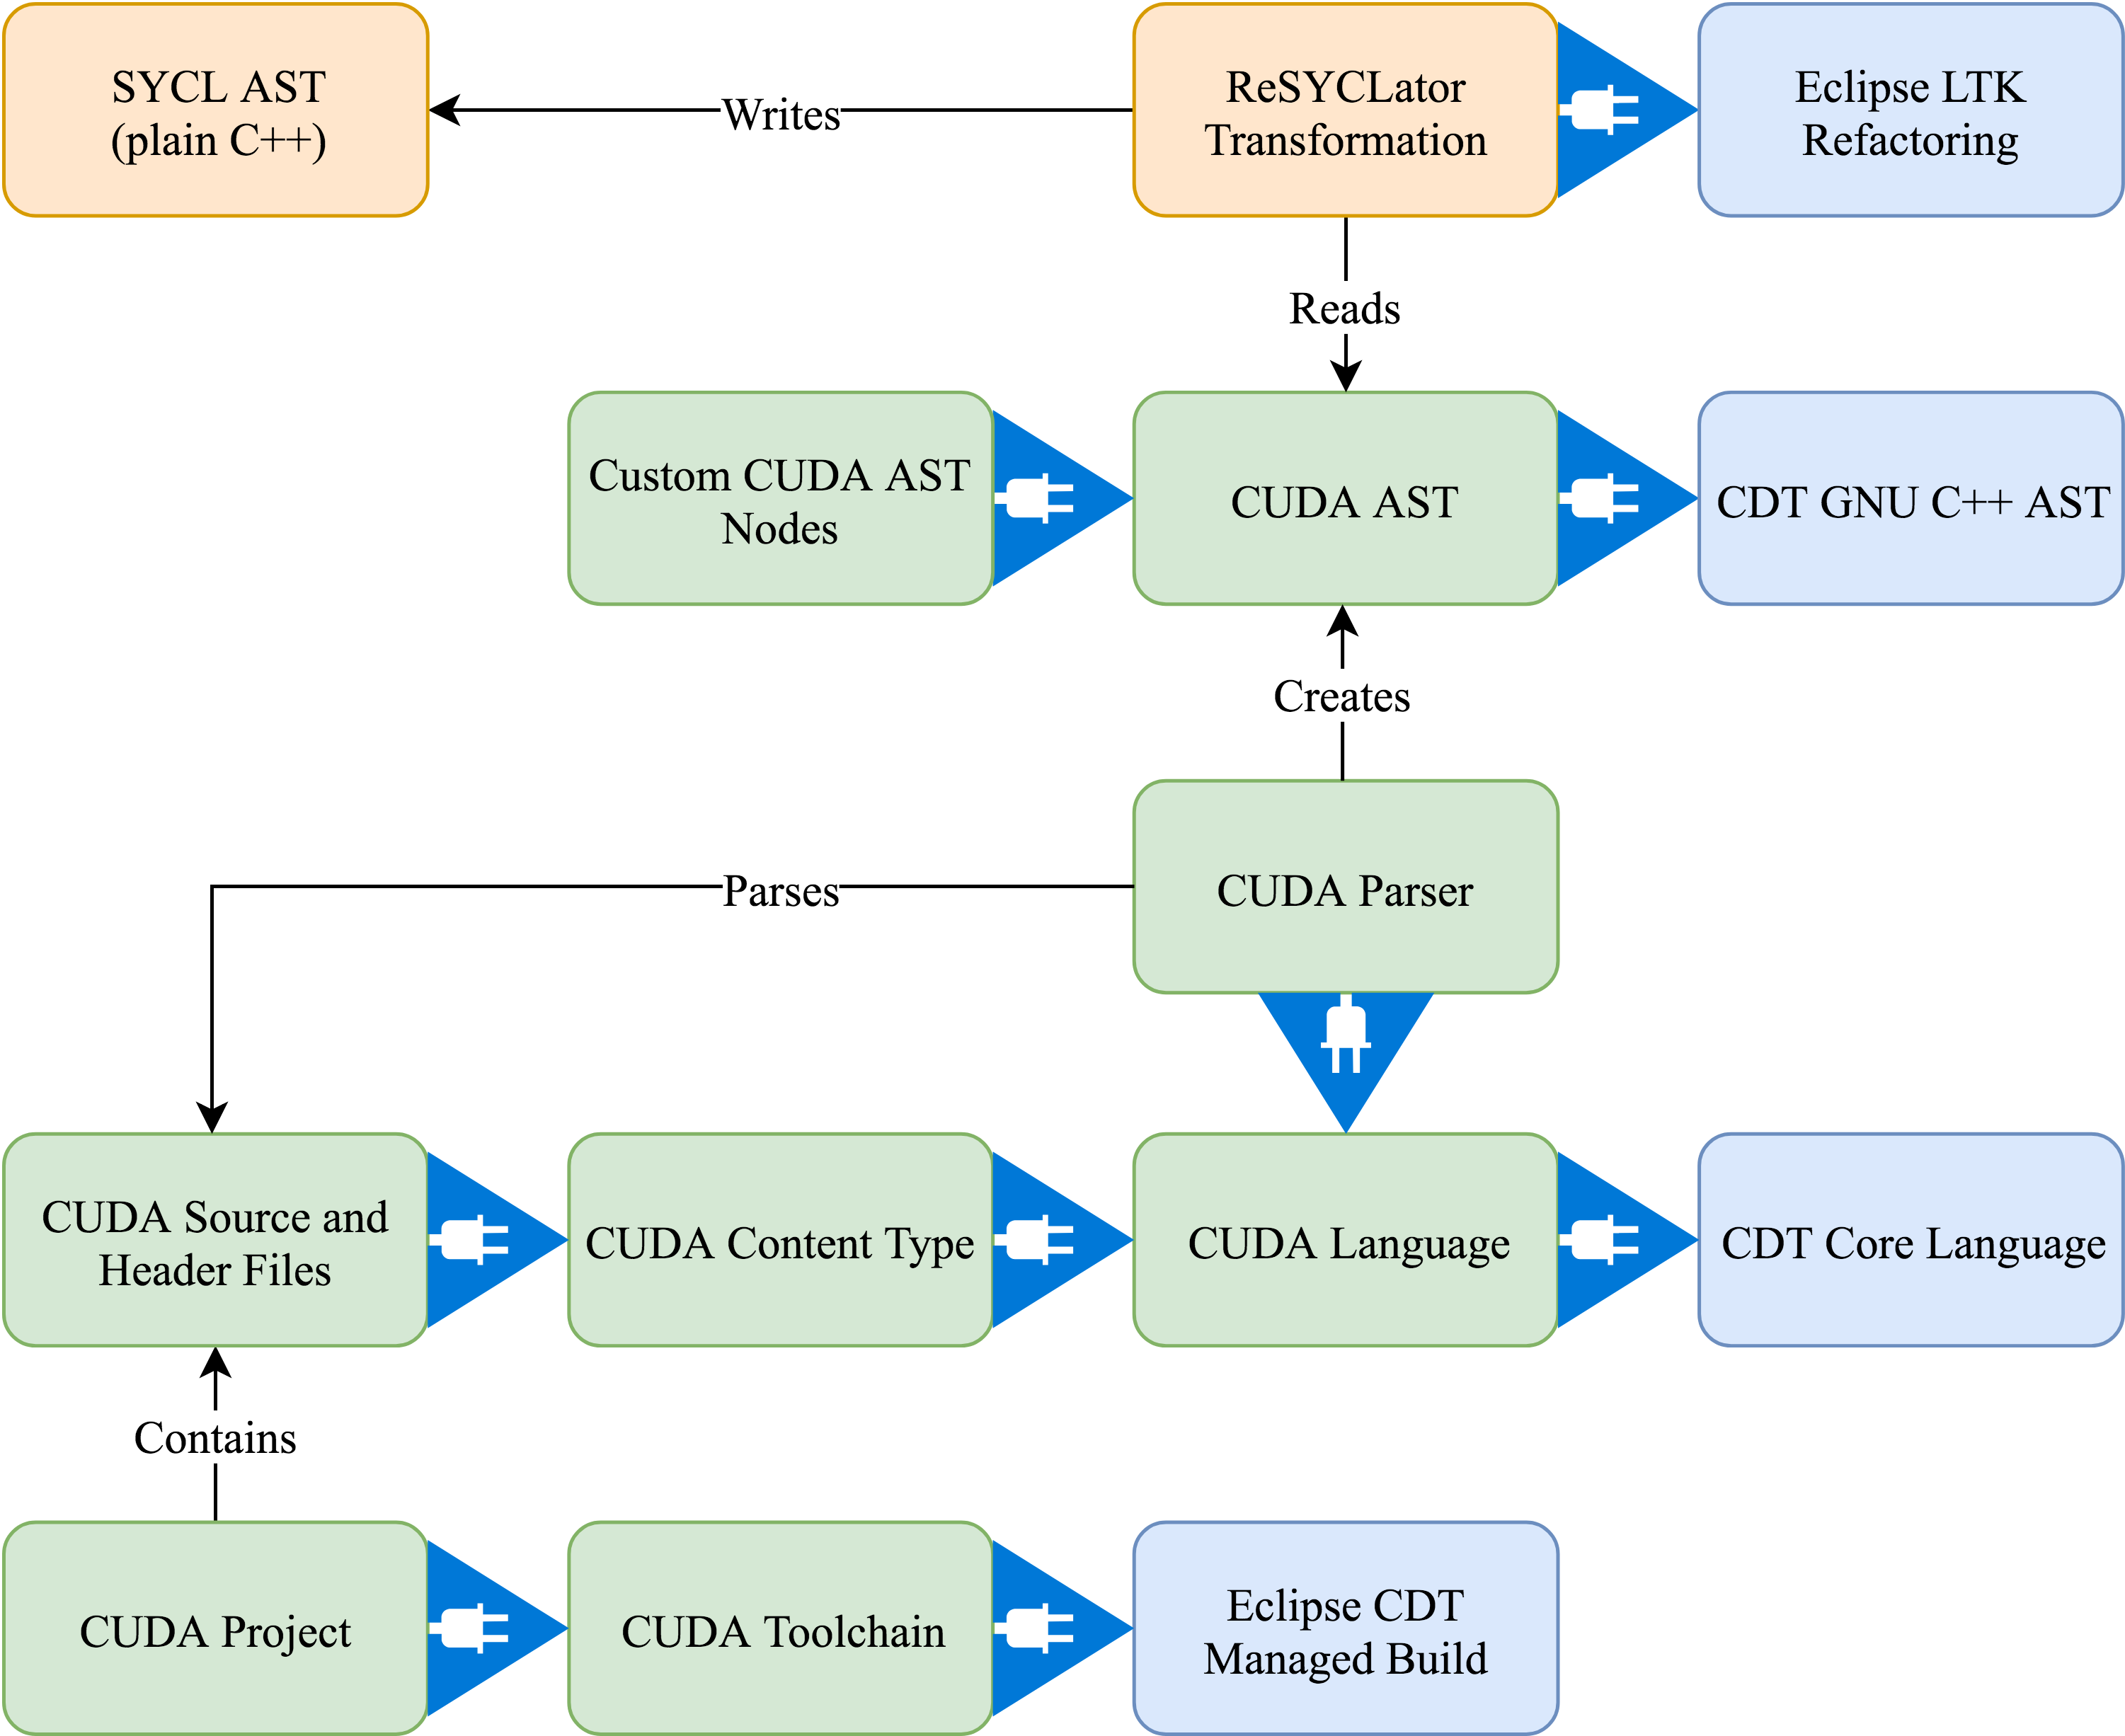
\includegraphics[width=\linewidth]{ResultSchemaSimple}
  \caption{Plug-in dependencies of CUDA C++ parser SYCL transformation. Triangles mark plug-in extensions.}
  %\Description{.}
  \label{fig:toolarch}
\end{figure}

\section{Outlook and Future Work}
Creating such tooling during a Master's degree fixed time frame requires omitting some desirable features. For example, creating SYCL kernels that directly rely on accessors instead of \tcode{global_ptr} is one of the omissions to be able to complete the transformation. The mapping of multiple dimensions within the kernel instead of the generated "pointer arithmetic" is another. But we believe the created infrastructure with its automated tests provides a good starting point for further productizing. The interactive nature under the control of the developer in an IDE allows to be only partially complete and still eases the porting, in contrast to an almost impossible fully automatic solution. 

A future product might provide SYCL-specific code analysis and refactoring options to suggest code improvements, e.g., for detecting sub-optimal SYCL mechanism usages, or for improving the generated SYCL code of a transformation. As of today, some existing C++ refactorings, such as "Extract using declaration" for qualified names, already can improve readability of the generated SYCL code that uses fully-qualified names for SYCL components.

More CUDA features, such as transforming CUDA streams to SYCL queues and more sophisticated management of selectors and devices. Also other memory regions, such as constant memory or CUDA's "write-to-symbol" mechanism, need to be handled by the transformation. 

As a side effect the CUDA parsing and AST infrastructure and its integration into the refactoring AST rewriting engine of Eclipse CDT will allow better IDE support for CUDA developers as well. 


%
% The acknowledgments section is defined using the "acks" environment (and NOT an unnumbered section). This ensures
% the proper identification of the section in the article metadata, and the consistent spelling of the heading.
\begin{acks}
To our Codeplay friends who inspired work on CUDA to SYCL transformation and their support during Tobias' master project work.
\end{acks}

%
% The next two lines define the bibliography style to be used, and the bibliography file.
\bibliographystyle{ACM-Reference-Format}
\bibliography{articleStauber}

% 
% If your work has an appendix, this is the place to put it.
\appendix
%\section{Appendices}

\section{Longer Code Examples}
\lstset{basicstyle=\footnotesize\ttfamily}
\inputcode{cuda-main.cpp}{\tcode{main()} calling CUDA matrix multiplication kernel}

\inputsycl{sycl-matrix-main.cpp}{Complete converted SYCL matrix multiplication}

\end{document}
